\documentclass{article}
\usepackage{graphicx} % Required for inserting images
\usepackage{amsmath}
\usepackage{amsfonts}
\usepackage{subcaption}
\usepackage{float} % Add this in your preamble

\title{Deep Learning: Homework 1 - Theory}
\author{Haotong Wu hw2933}
\date{February 2024}

\begin{document}

\maketitle

\subsection*{1.1 Two-Layer Neural Nets}

\subsubsection*{1.1.1 Regression Task}

We would like to perform a regression task. We choose $f(\cdot) = 3(\cdot)^+ = 3$ReLU$(\cdot)$ and $g$ to be the identity function. To train this network, we want to minimize the energy loss $L$ and this is computed via the squared Euclidean distance cost $C$, such that $L(w, x, y) = F(x, y) = C(y, \tilde{y}) = \|\tilde{y} - y\|^2$, where $y$ is the output target.


\begin{itemize}
    \item[(a)] (1pt) Name and mathematically describe the 5 programming steps you would take to train this model with PyTorch using SGD on a single batch of data.
    \subsection*{Answer.}
    \begin{enumerate}
    \item Generate a prediction model and get the prediction of $y$.  $\tilde{y} = \text{model}(x)$
    \item Compute the loss with respect to the outputs. $L(w, x, y) = F(x, y) = C(y, \tilde{y}) = \|\tilde{y} - y\|^2$
    \item  Zeroing the gradient of the parameters, initialize the gradient for the next step. 
    \item Backward propagate the gradients back through the network using the chain rule to compute the gradients \(\frac{\partial L}{\partial W^{(1)}}, \frac{\partial L}{\partial b^{(1)}}, \frac{\partial L}{\partial W^{(2)}}, \frac{\partial L}{\partial b^{(2)}}\).
    \item Update the parameters in the direction opposite to the gradient, scaled by the learning rate.
    \end{enumerate}
    
    \item[(b)] (4pt) For a single data point $(x, y)$, write down all inputs and outputs for forward pass of each layer. You can only use variable $x, y, W^{(1)}, b^{(1)}, W^{(2)}, b^{(2)}$ in your answer. (note that Linear$_i(x) = W^{(i)}x + b^{(i)}$).
    \subsection*{Answer.}
    \begin{enumerate}
        \item Linear layer 1: INPUT: $\boldsymbol{x}$ OUTPUT: $s_1 = \boldsymbol{{W}^{(1)}}\boldsymbol{x} + \boldsymbol{{b}^{(1)}}$ \\
        $f$ function: INPUT: $s_1 = \boldsymbol{{W}^{(1)}}\boldsymbol{x} + \boldsymbol{{b}^{(1)}}$ OUTPUT: $a_1 = f(s_1) = 3\text{ReLU}(s_1) = 3\text{ReLU}(\boldsymbol{{W}^{(1)}}\boldsymbol{x} + \boldsymbol{{b}^{(1)}})$
        \item Linear layer 2: INPUT: $3\text{ReLU}(\boldsymbol{{W}^{(1)}} \boldsymbol{x} + \boldsymbol{{b}^{(1)}})$ OUTPUT: $s_2 = \boldsymbol{{W}^{(2)}}3\text{ReLU}(\boldsymbol{{W}^{(1)}}\boldsymbol{x} + \boldsymbol{{b}^{(1)}}) + \boldsymbol{{b}^{(2)}}$\\
        $g$ identity function: INPUT: $\boldsymbol{{W}^{(2)}}3\text{ReLU}(\boldsymbol{{W}^{(1)}}\boldsymbol{x} + \boldsymbol{{b}^{(1)}}) + \boldsymbol{{b}^{(2)}}$ OUTPUT: $\tilde{y} = g(s_2) = \boldsymbol{{W}^{(2)}}3\text{ReLU}(\boldsymbol{{W}^{(1)}}\boldsymbol{x} + \boldsymbol{{b}^{(1)}}) + \boldsymbol{{b}^{(2)}}$
    \end{enumerate}
    
    
    \item[(c)] (6pt) Write down the gradients calculated from the backward pass. You can only use the following variables: $x, y, W^{(1)}, b^{(1)}, W^{(2)}, b^{(2)}, \frac{\partial C}{\partial \tilde{y}}, \frac{\partial a_1}{\partial s_1}, \frac{\partial \tilde{y}}{\partial s_2}$ in your answer, where $s_1, a_1, s_2, \tilde{y}$ are the outputs of Linear$_1, f, $ Linear$_2, g$.
    
    
     \subsection*{Answer.}
      $\tilde{y} \rightarrow s_2 \rightarrow a_1 \rightarrow s_1 \rightarrow x$
     \begin{enumerate} 
     \item \(\frac{\partial \mathcal{C}}{\partial \boldsymbol{{W^{(2)}}}} = \frac{\partial \mathcal{C}}{\partial \tilde{y}} \frac{\partial \tilde{y}}{\partial s_{2}} \frac{\partial s_{2}}{\partial W^{(2)}} = \frac{\partial \mathcal{C}}{\partial \tilde{y}} \frac{\partial \tilde{y}}{\partial s_{2}} a_1 
     =\frac{\partial \mathcal{C}}{\partial \tilde{y}} \frac{\partial \tilde{y}}{\partial s_{2}}3\textbf{ReLU}(W^{(1)}x + b^{(1)})  \)
    \item \(\frac{\partial \mathcal{C}}{\partial b^{(2)}} = \frac{\partial \mathcal{C}}{\partial \tilde{y}} \frac{\partial \tilde{y}}{\partial s_{2}} \frac{\partial s_{2}}{\partial b^{(2)}} = \frac{\partial \mathcal{C}}{\partial \tilde{y}} \frac{\partial \tilde{y}}{\partial s_{2}}\)
    \item \(\frac{\partial \mathcal{C}}{\partial W^{(1)}} = \frac{\partial \mathcal{C}}{\partial \tilde{y}} \frac{\partial \tilde{y}}{\partial s_{2}} \frac{\partial s_{2}}{\partial a_{1}} \frac{\partial a_{1}}{\partial s_{1}} \frac{\partial s_{1}}{\partial W^{(1)}} =  \frac{\partial \mathcal{C}}{\partial \tilde{y}} \frac{\partial \tilde{y}}{\partial s_{2}} W^{(2)} \frac{\partial a_{1}}{\partial s_{1}} x \)
    
    \item \(\frac{\partial \mathcal{C}}{\partial b^{(1)}} = \frac{\partial \mathcal{C}}{\partial \tilde{y}} \frac{\partial \tilde{y}}{\partial s_{2}} \frac{\partial s_{2}}{\partial a_{1}} \frac{\partial a_{1}}{\partial s_{1}} \frac{\partial s_{1}}{\partial b^{(1)}} = \frac{\partial \mathcal{C}}{\partial \tilde{y}} \frac{\partial \tilde{y}}{\partial s_{2}} W^{(2)} \frac{\partial a_1}{\partial s_{1}} \)
     \end{enumerate}
    

        
  
        
    \item[(d)] (2pt) Show us the elements of $\frac{\partial a_1}{\partial s_1}, \frac{\partial \tilde{y}}{\partial s_2}$ and $\frac{\partial C}{\partial \tilde{y}}$ (be careful about the dimensionality)?
    \subsection*{Answer.}
    \item From the ReLU function, we have:
    \[a_1 = 
    \begin{cases}
    3s_1 & \text{if } s_{1} > 0 \\
    0 & \text{if } s_{1} \leq 0
    \end{cases}
    \]
    Then, we can derive that 
    \[ \frac{\partial a_1}{\partial s_1} = 
    \begin{cases}
    3 & \text{if } s_{1} > 0 \\
    0 & \text{if } s_{1} \leq 0
    \end{cases}
    \in \mathbb{R}^{D}
    \]
    
    \item Since \(g\) is the identity function, the derivative of \(\tilde{y}\) with respect to \(s_2\) is 1:
    \[ \frac{\partial \tilde{y}}{\partial s_2} = I \in \mathbb{R}^{K \times K} \]
    where \(I\) is the identity matrix of size \(K \times K\).
    
    \item For the derivative of the cost function \(C\) with respect to \(\tilde{y}\), given the squared Euclidean distance cost, we have:
    \[ \frac{\partial C}{\partial \tilde{y}} = \frac{\partial}{\partial \tilde{y}} \| \tilde{y} - y \|_2^2 \]
    Expanding the norm squared, we get:
    \[ \frac{\partial C}{\partial \tilde{y}} = 2 (\tilde{y} - y) \in \mathbb{R}^{1 \times K} \]
    which indicates that the gradient of the cost function with respect to each element of the prediction vector \(\tilde{y}\) is simply twice the element-wise difference between \(\tilde{y}\) and \(y\), in \(\mathbb{R}^K\).
    
\end{itemize}

\subsubsection*{1.1.2 Classification Task}

We would like to perform a multi-class classification task, so we set $f = \tanh$ and $g = \sigma$, the logistic sigmoid function $\sigma(x) = ({1 + \exp(-x)})^{-1}$.


\begin{itemize}
    \item[(a)] (2pt + 3pt + 1pt) If you want to train this network, what do you need to change in the equations of (b), (c) and (d), assuming we are using the same squared Euclidean distance loss function.
    \subsection*{Answer.}
    \begin{enumerate}
        \item{Changes in (b) Forward Pass Equations:}\\
        For $f = \tanh$, replace the $f$ function step with:
        \[ a_1 = f(s_1) = \tanh(s_1) = \tanh(W^{(1)}x + b^{(1)}) \]
        For \(g = \sigma\), replace the \(g\) identity function step with:
        \[ \tilde{y} = g(s_2) = \sigma(s_2) = \frac{1}{1 + \exp(-s_2)}  \]
        \item {Changes in (c) Backward Pass Equations:} \\
        There is no change in the backward pass equations, only the function changes, but they use the same equations.
        \item{Changes in (d):}\\
        % \[\frac{\partial a_1}{\partial s_1} = 1 - \text{tanh}^2(s_1)\]\\
        % \[\frac{\partial \tilde{y}}{\partial s_2} = \sigma(s_1)\cdot (1- \sigma(s_1))\]
        The derivative \( \frac{\partial a_1}{\partial s_1} \) is a diagonal matrix of dimension \( m \times m \), where each diagonal element is \( 1-\tanh^2((s_1)_i) \).
        The derivative \( \frac{\partial \tilde{y}}{\partial s_2} \) is a diagonal matrix of dimension \( K \times K \), where each diagonal element is \( \sigma((s_2)_i)(1 - \sigma((s_2)_i)) \).

    \end{enumerate}



    
    \item[(b)] (2pt + 3pt + 1pt) Now you think you can do a better job by using a Binary Cross Entropy (BCE) loss function $D_{\text{BCE}}(y, \tilde{y}) = \frac{1}{K} \sum_{i=1}^{K} -[y_i \log(\tilde{y}_i) + (1 - y_i) \log(1 - \tilde{y}_i)]$. What do you need to change in the equations of (b), (c) and (d)?
    \subsection*{Answer.}
    \begin{enumerate}
        \item{Changes in (b) Forward Pass Equations:}\\
        There is no change in the forward pass equations, only the loss function changes.
        \item {Changes in (c) Backward Pass Equations:} \\
         Since the loss function changes, the derivative of the loss function with respect to the output \(\tilde{y}\) will change. 
         And also other derivatives with loss function will change accordingly.       
        \item{Changes in (d):}\\
        The derivative \( \frac{\partial a_1}{\partial s_1} \) is a diagonal matrix of dimension \( m \times m \), where each diagonal element is \( 1-\tanh^2((s_1)_i) \).
        The derivative \( \frac{\partial \tilde{y}}{\partial s_2} \) is a diagonal matrix of dimension \( K \times K \), where each diagonal element is \( \sigma((s_2)_i)(1 - \sigma((s_2)_i)) \).
        The derivative \( \frac{\partial C}{\partial \tilde{y}} \in \mathbb{R}^{1 \times K} \) will change to: 
        \[\left( \frac{\partial \mathcal{C}}{\partial \tilde{y}} \right)_{i} = \frac{1}{K} \left( \frac{y_i - \tilde{y}_i}{\tilde{y}_i (\tilde{y}_i - 1)} \right)
\]

        
    \end{enumerate}



    \item[(c)] (1pt) Things are getting better. You realize that not all intermediate hidden activations need to be binary (or soft version of binary). You decide to use $f(\cdot) = (\cdot)^+ $ but keep $g$ as $\sigma$. Explain why this choice of $f$ can be beneficial for training a (deeper) network.
    \subsection*{Answer.}
    Because \(f(\cdot) = (\cdot)^+\) allows the network to learn more complex functions. 
    The ReLU function is non-linear and has a simple derivative, which makes it computationally efficient. 
    And it also helps to mitigate the vanishing gradient problem, which can occur in deeper networks when using the sigmoid or tanh activation functions. 
    Additionally, it can also less computationally expensive than other functions such as sigmoid and tanh, which can be beneficial for training deeper networks.
\end{itemize}

\subsection*{1.2 Conceptual Questions}

\begin{itemize}
    \item[(a)] (1pt) Why is softmax actually softargmax?
 \subsection*{Answer.}
    The softmax function is a differentiable approximation of the argmax function. 
    The softargmaxargmax function is a non-differentiable function that returns the index of the maximum value in a tensor. 
    \item[(b)] (3pt) Draw the computational graph defined by this function, with inputs $x, y, z \in \mathbb{R}$ and output $w \in \mathbb{R}$. You make use symbols $x, y, z, o$, and operators $*, +$ in your solution. Be sure to use the correct shape for symbols and operators as shown in class.

\[ a = x * y + z \]
\[ b = a * (x + x) \]
\[ w = a * b + b \]
\subsection*{Answer.}
\begin{figure}[H]
    \centering
    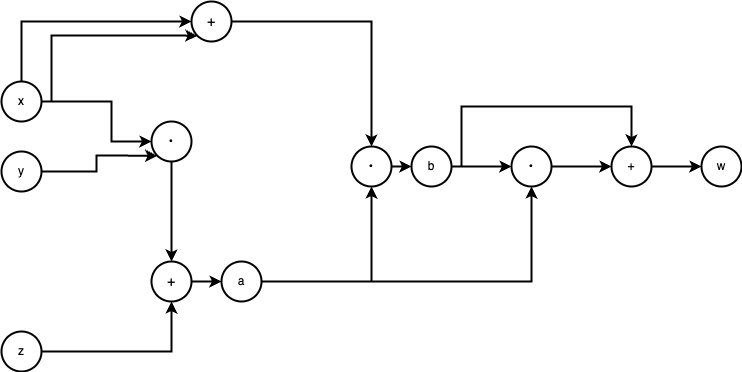
\includegraphics[width=0.8\textwidth]{image.png}
    \caption{Computational Graph}
    \label{fig:computational_graph}
\end{figure}


    \item[(c)] (2pt) Draw the graph of the derivative for the following functions:

        \item GELU()
        \item LeakyReLU (negative\_slope=0.1)
        \item ReLU()
        \item Tanh()
    % \end{itemize}

    \subsection*{Answer.}
    \begin{figure}[H]
        \centering
        \begin{subfigure}[b]{0.45\textwidth} % Adjust the width as needed
          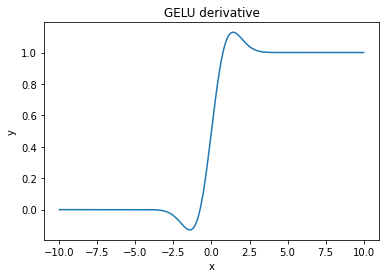
\includegraphics[width=\textwidth]{GELU.png}
          \caption{GELU}
          \label{fig:GELU}
        \end{subfigure}
        \hfill % This will add some spacing between your subfigures
        \begin{subfigure}[b]{0.45\textwidth} % Adjust the width as needed
          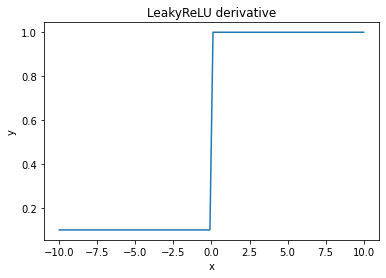
\includegraphics[width=\textwidth]{lrelu.png}
          \caption{LeakyReLU}
          \label{fig:LeakyReLU}
        \end{subfigure}
        % You can add a \newline or \vspace here if you want to adjust the spacing between the rows
        \newline % This will ensure the next pair of subfigures appears on the next line
        \begin{subfigure}[b]{0.45\textwidth} % Adjust the width as needed
          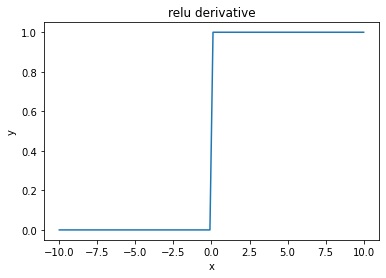
\includegraphics[width=\textwidth]{relu.png}
          \caption{ReLU}
          \label{fig:ReLU}
        \end{subfigure}
        \hfill % This will add some spacing between your subfigures
        \begin{subfigure}[b]{0.45\textwidth} % Adjust the width as needed
          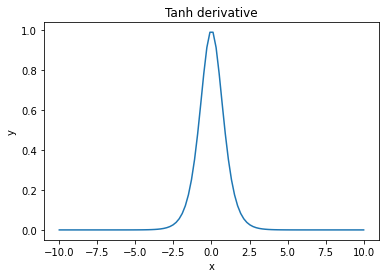
\includegraphics[width=\textwidth]{tanh.png}
          \caption{Tanh}
          \label{fig:Tanh}
        \end{subfigure}
        \caption{Graphs}
        \label{fig:activation_functions}
      \end{figure}
      

    \item[(d)] (3pt) Given function $f(x) = W_1 x$ with $W_1 \in \mathbb{R}^{b \times a}$ and $g(x) = W_2 x$ with $W_2 \in \mathbb{R}^{b \times a}$:
    \begin{enumerate}
        \item What is the Jacobian matrix of $f$ and $g$
        \item What is the Jacobian matrix of $h(x) = f(x) + g(x)$
        \item What is the Jacobian matrix of $h(x) = f(x) + g(x)$ if $W_1 = W_2$
    \end{enumerate}
    \subsection*{Answer.}
    \begin{enumerate}
        \item The Jacobian matrix of \(f\) is \(\frac{\partial f}{\partial x} = \boldsymbol{{W_1} \in} \mathbb{R}^{b \times a}\).\\
        And the Jacobian matrix of \(g\) is \(\frac{\partial g}{\partial x} = \boldsymbol{{W_2} \in} \mathbb{R}^{b \times a}\)..
        \item The Jacobian matrix of \(h(x) = f(x) + g(x)\) is \(\frac{\partial h}{\partial x} = \frac{\partial (f(x) + g(x))}{\partial x} = \frac{\partial f}{\partial x} + \frac{\partial g}{\partial x} = \boldsymbol{{W_1} + \}boldsymbol{{W_2} \in} \mathbb{R}^{b \times a}\).
        \item If \(W_1 = W_2\), then the Jacobian matrix of \(h(x) = f(x) + g(x)\) is \(2\boldsymbol{{W_1} \in} \mathbb{R}^{b \times a}\) or \(2\boldsymbol{{W_2} \in} \mathbb{R}^{b \times a}\)
    \end{enumerate}
    
    
    \item[(e)] (3pt) Given function $f(x) = W_1 x$ with $W_1 \in \mathbb{R}^{b \times a}$ and $g(x) = W_2 x$ with $W_2 \in \mathbb{R}^{c \times b}$:
    \begin{enumerate}
        \item What is the Jacobian matrix of $f$ and $g$
        \item What is the Jacobian matrix of $h(x) = g(f(x)) = (g \circ f)(x)$
        \item What is the Jacobian matrix of $h(x)$ if $W_1 = W_2$ (so $a = b = c$)
    \end{enumerate}
    \subsection*{Answer.}
    \begin{enumerate}
        \item The Jacobian matrix of \(f\) is \(\frac{\partial f}{\partial x} = \boldsymbol{{W_1} \in} \mathbb{R}^{b \times a}\).\\
        And the Jacobian matrix of \(g\) is \(\frac{\partial g}{\partial x} = \boldsymbol{{W_2} \in} \mathbb{R}^{c \times b}\)..
        \item The Jacobian matrix of \(h(x) = g(f(x))\) is \(\frac{\partial h}{\partial x} = \frac{\partial g(f(x))}{\partial x} = \frac{\partial g}{\partial x} \frac{\partial f}{\partial x} = \boldsymbol{{W_2} \bo}ldsymbol{{W_1} \in} \mathbb{R}^{c \times a}\).
        \item If \(W_1 = W_2\), then we can know that \(a = b = c\), and the Jacobian matrix of \(h(x) = g(f(x))\) is \(\boldsymbol{{W_1} \bo}ldsymbol{{W_1} \in} \mathbb{R}^{a \times a}\) or \(\boldsymbol{{W_2} \bo}ldsymbol{{W_2} \in} \mathbb{R}^{c \times c}\)
    \end{enumerate}



\end{itemize}

\section*{1.3 Deriving Loss Functions}

Derive the loss function for the following algorithms based on their common update rule $w_i \leftarrow w_i + \eta (y - \tilde{y}) x_i$. Show the steps of the derivation given the following inference rules (simply stating the final loss function will receive no points).

\begin{enumerate}
    \item (4 points) Perceptron: $\tilde{y} = \text{sign}(b + \sum_{i=1}^{d} w_i x_i)$
    \item (4 points) Adaline / Least Mean Squares: $\tilde{y} = b + \sum_{i=1}^{d} w_i x_i$
    \item (4 points) Logistic Regression: $\tilde{y} = \tanh(b + \sum_{i=1}^{d} w_i x_i)$
\end{enumerate}

% \subsection*{Answer.}
% \begin{enumerate}
%     \item Perceptron: $\tilde{y} = \text{sign}(b + \sum_{i=1}^{d} w_i x_i)$\\
%     Step:
%     \[ L(x, y, w) = -(y - \tilde{y}) \sum_{j=1}^{d} w_j x_j\]
%     \item Adaline / Least Mean Squares: $\tilde{y} = b + \sum_{i=1}^{d} w_i x_i$\\
%     Step:
%     \[L(x, y, w) = \frac{1}{2} (y - \tilde{y})^2 = \frac{1}{2} \left(y - \sum_{i=1}^{d} w_i x_i\right)^2\]

%     \item Logistic Regression: $\tilde{y} = \tanh(b + \sum_{i=1}^{d} w_i x_i)$\\
%     Step:
%     \[L(x, y, w) = -2\log\left(1 + \exp\left(-y \sum_{j=1}^{d} w_j x_j\right)\right)\]
      
% \end{enumerate}
\subsection*{Answer.}
\begin{enumerate}
    \item Perceptron: $\tilde{y} = \text{sign}(b + \sum_{i=1}^{d} w_i x_i)$
    \begin{itemize}
        \item The Perceptron uses a step function for activation which outputs either +1 or -1.
        And our goal is to minimize the number of misclassified points.
        When the prediction $\tilde{y}$ matches the actual label $y$, there is no loss.
        Otherwise, we incur a loss which should push the weights to correct the classification.
        The loss function for a misclassified point is proportional to the distance from the decision boundary, which is given by $\sum_{i=1}^{d} w_i x_i$.
        This leads to the loss function $L(x, y, w) = - (y - \tilde{y}) \sum_{i=1}^{d} w_i x_i$ for a misclassified point.
    \end{itemize}

    \item Adaline / Least Mean Squares: $\tilde{y} = b + \sum_{i=1}^{d} w_i x_i$
    \begin{itemize}
        \item Adaline uses a linear activation function, and
        the goal is to minimize the squared error between the prediction and the actual value.
        The squared error has a gradient that points in the direction of the steepest descent in the error surface.
        This is captured by the loss function \[L(x, y, w) = \frac{1}{2} (y - \tilde{y})^2 = \frac{1}{2} \left(y - \sum_{i=1}^{d} w_i x_i\right)^2\]
        which is differentiable and convex.
        The factor of $\frac{1}{2}$ simplifies the gradient, making it cleaner when we take the derivative with respect to $w_i$.
    \end{itemize}

    \item Logistic Regression: $\tilde{y} = \tanh(b + \sum_{i=1}^{d} w_i x_i)$
    \begin{itemize}
        \item Logistic Regression is used for binary classification, and $\tanh$ serves as a smooth, differentiable approximation to the step function.
        The output of $\tanh$ is bounded between -1 and 1, similar to the labels in binary classification.
        The loss function is derived from the negative log-likelihood of the Bernoulli distribution.
        We can derive the loss function as \[L(x, y, w) = -2\log\left(1 + \exp\left(-y \sum_{j=1}^{d} w_j x_j\right)\right)\]
        The partial derivatives with respect to $w_i$ and $b$ indicate how the weights should be updated to minimize the loss.
    \end{itemize}
\end{enumerate}

\end{document}

\end{document}